\subsection{Clustering design}
\label{sec:clusteringDesign}

\subsubsection{Conceptual basis}
Regular expression languages are infinite and exhibit substantial variety, but programmers are likely to use them for a limited number of purposes.  The goal of this study is to identify categories of regular expression usage and the frequency of usage in these categories so that designers of regular expression languages and end-user tools can better support what is most useful to programmers.  In this study, a regex similarity measurement technique was devised and used to group regex with similar behavior into clusters.  The clusters representing the most projects were then in turn manually grouped into general categories of behavior.

% This study employs a sequence of two categorization attempts to achieve its goal.
% \begin{itemize}\itemsep -1pt
% \item[1] determine an objective behavioral similarity score for all pairs of regexes, and find clusters of highly similar regexes, so that a large number of regexes can be seen as a modest number of clusters, and then manually categorize these clusters
% \item[2] using the categories from step 1 as a guide in understanding how behavior will cluster, create a categorization technique by iterative attempts and then manually categorize regexes based on inspection alone
% \end{itemize}

\subsubsection{Determining behavioral similarity}
An ideal analysis of regex behavioral similarity would use subsumption or containment analysis. However, a tool that could facilitate such an analysis of the corpus could not be found.  For this reason, a new technique using string matching was developed that can create a similarity score between two regexes with existing technology.

\begin{figure}[tb]
\centering
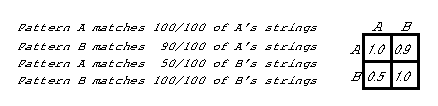
\includegraphics[height=0.85in]{nontex/illustrations/minimalMatrix.eps}
\caption{A similarity matrix created by counting strings matched}
\label{fig:minimalMatrix}
\end{figure}

\begin{figure}[tb]
\centering
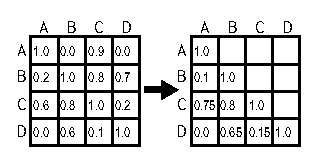
\includegraphics[width=0.5\columnwidth]{nontex/illustrations/matrixToGraph.eps}
\vspace{-6pt}
\caption{Creating a similarity graph from a similarity matrix}
\vspace{-6pt}
\label{fig:matrixToGraph}
\end{figure}



\subsubsection{Building a similarity matrix}
The similarity analysis used in this study clusters regular expressions by their behavioral similarity on matched strings.  Consider two unspecified regexes \cverb!A! and \cverb!B!.
Now consider a set of 100 strings that match \cverb!A!, named \underline{\tt A100m}.  If \cverb!B! matches 90 strings in \underline{\tt A100m}, then If \cverb!B! is 90\% similar to If \cverb!A!.  Similarly, consider a set of 100 strings that match \cverb!B!, named \underline{\tt B100m}.  If \cverb!A! matches 50 strings in \underline{\tt B100m}, then If \cverb!A! is 50\% similar to If \cverb!B!.  Notice that by this definition, each regex is 100\% similar to itself.  Similarity scores are used to create a similarity matrix as shown in Figure~\ref{fig:minimalMatrix}.

Once the similarity matrix is built, the values of cells reflected across the diagonal of the matrix are averaged to create a half-matrix of undirected similarity edges, as illustrated in Figure~\ref{fig:matrixToGraph}.
This facilitates clustering using the  Markov Clustering (MCL) algorithm\footurl{http://micans.org/mcl/}.
MCL was chosen because it offers a fast and tunable way to cluster items by similarity and it is particularly useful when the number of clusters is not known \emph{a priori}.


In the implementation, strings are generated for each regex using Rex~\cite{rex}.  Rex generates matching strings by representing the regular expression as an automaton, and then passing that automation to a constraint solver that generates members for it\footurl{http://research.microsoft.com/en-us/projects/rex/}.  If the regex matches a finite set of strings smaller than 400, Rex will produce a list of all possible strings.
In this study, the goal is to generate 400 strings for each regex to balance the runtime of the similarity analysis with the precision of the similarity calculations.

For clustering, the similarity matrix is pruned to retain all similarity values greater than or equal to 0.75, setting the rest to zero, and then using MCL.
This threshold was selected based on recommendations in the MCL manual. The impact of lowering the threshold would likely result  in either the same number of more diverse clusters, or a larger number of clusters, but is unlikely to markedly change the largest clusters or their summaries.
We also note that MCL can also be tuned using many parameters, including inflation and filtering out all but the top-k edges for each node.
After exploring the quality of the clusters using various tuning parameter combinations, the best clusters (by inspection) were found using an inflation value of 1.8 and k=83.   The top 100 clusters are categorized by inspection into six categories of behavior.

The end result is clusters and categories of highly behaviorally similar regular expressions, though this approach has a tendency to over-approximate the similarity of two regexes. Similarity is measured based on a finite set of generated strings, but some regexes match an infinite set (e.g., \cverb!ab*c!), so measuring similarity based on the first 400 strings may lead to an artificially high similarity value. To mitigate this threat, a large number of generated strings was used for each regex, but future work includes exploring other approaches to computing regex similarity.
